\label{chapter:conceitos}
Este capítulo tem apresenta os principais conceitos e definições abordados neste trabalho, tais como: Linguagens de descrição de hardware, Verificação de sistemas e Técnicas de Compiladores.

%============================
%Linguagens de descrição de hardware
%============================
\section{Linguagens de descrição de hardware}

As linguagens de descrição de hardware (HDL) foram desenvolvidas com o intuito de auxiliar a criação de circuitos lógicos com grande número de elementos e com uma gama de abstrações lógicas e eletrônicas~\cite{thomas2008verilog}. \textcolor{red}{Entre os exemplos, podemos citar: \textit{VDHL}~\cite{IEEEVHDLLanguage}, \textit{Verilog}~\cite{IEEEVerilogLanguage} e \textit{SystemC}~\cite{IEEESystemCLanguage}.}

\par
Segundo~\citeonline{christen1999vhdl}, linguagens de descrição de hardware são linguagens de programação utilizadas com o intuito de descrever o comportamento de um determinado circuito, técnica conhecida como modelagem. Os modelos descritos em HDL são utilizados como entrada para um simulador, onde o mesmo pode ter seu comportamento analisado.

\par
As HDL's trazem consigo diversas vantagens, entre elas códigos independentes de tecnologia e fabricante, podendo ser portáteis e reutilizáveis \cite{cappelattipraticando}. As linguagens mais modernas, tais como VHDL e \textit{Verilog}, possuem suporte tanto a descrição do circuito propriamente dito, quanto ao comportamento que o mesmo deve exercer \cite{christen1999vhdl}.

\par
A \textit{Verilog}, como já citado, é uma linguagem de descrição de \textit{hardware} que fornece diversos níveis de abstração para desenvolvimento de sistemas digitais\cite{thomas2008verilog}. A linguagem foi desenvolvida para ser simples e efetiva nos diversos níveis de abstração incluindo o suporte ao desenvolvimento, verificação, síntese e testes de \textit{software}~\cite{IEEEVerilogLanguage}.

\begin{figure}[H]
\caption{\label{fig:mux_verilog} Exemplo de multiplexador descrito em Verilog.}
	\begin{center}
    \begin{minipage}{0.7\textwidth}
    \begin{lstlisting}       
primitive multiplexer (mux, control, dataA, dataB);
output mux;
input control, dataA, dataB;
endprimitive
\end{lstlisting}
    \end{minipage}
	\end{center}
    \legend{Fonte: Adaptado de~\cite{IEEEVerilogLanguage}.}
\end{figure}

\par
\textcolor{red}{Na \autoref{fig:mux_verilog} apresenta um exemplo de multiplexador descrito em \textit{Verilog} utilizando a estrutura de modelagem, chamada \textit{UDP} que permite a criação de novos primitivas para serem utilizada. Apresenta uma saída apenas(mux) e três entradas sendo uma de controle(control) e duas de dados(dataA e dataB).}

\par
A VHDL é uma linguagem de descrição de hardware amplamente utilizada, concebida na década de 80, devido uma necessidade do Departamento de Defesa dos Estados Unidos da América~\cite{cappelattipraticando}. Assim como a Verilog, esta linguagem também suporta o desenvolvimento, a verificação, a síntese, e os testes de \textit{hardware}~\cite{IEEEVHDLLanguage}.

\begin{figure}[H]
\caption{\label{fig:mux_vhdl} Exemplo de multiplexador descrito em VHDL.}
	\begin{center}
    \begin{minipage}{0.6\textwidth}
    \begin{lstlisting}       
library IEEE;
use IEEE.std_logic_1164.all;
use IEEE.std_logic_unsigned.all;
entity mux2x1 is
port (sel: in STD_LOGIC;
      a,b: in STD_LOGIC;
      y: out STD_LOGIC);
end mux2x1;

architecture dataflow of mux2x1 is begin
y <= (a AND NOT sel) OR (b AND sel);
end dataflow.
\end{lstlisting}
    \end{minipage}
	\end{center}
    \legend{Fonte: \cite{cappelattipraticando}.}
\end{figure}

\par
\textcolor{red}{Na \autoref{fig:mux_vhdl} está descrito um multiplexador de duas entradas descrito em VHDL, apresentando na parte inicial as bibliotecas e na entidade(entity) a declaração das variáveis utilizadas. Na arquitetura(architecture) apresenta o funcionamento do multiplexador, relacionando entradas e saídas conforme tenham sido declarados. Este conceitos serão melhor apresentados na \autoref{sec:vhdl_seção}.}

\par
\textcolor{red}{Conforme apresentado nas \autoref{fig:mux_verilog} e \autoref{fig:mux_vhdl}, ambas as linguagens apresentam diferenças no modelos de declaração e utilização para descrição de hardware. Para este trabalho foi escolhido a VHDL devido a linguagem apresentar um melhor escopo para análise, facilitando o trabalho de análise proposto para este projeto.}


%Ambas as linguagens apresentam similaridades, sendo a linguagem VHDL escolhida para este trabalho devido a linguagem apresentar maior gama de recursos tanto para o desenvolvimento quanto para o auxílio nos testes\todo{Apresentar um exemplo com referência}.


%============================
%VHDL
%============================
\subsection{\label{sec:vhdl_seção}VHSIC Hardware Description Language - VHDL}
VHDL é uma linguagem de descrição de hardware destinada a ser utilizada em todas as etapas da criação de sistemas eletrônicos, sendo elas: desenvolvimento; verificação; síntese; e, teste de circuitos~\cite{IEEEVHDLLanguage}.
% 
Segundo~\citeonline{cappelattipraticando}, a VHDL apresenta três principais pilares: \textbf{abstração}, que consiste na descrição com diferentes níveis de detalhes; \textbf{modularidade}, que permite a divisão do projeto em vários blocos ou módulos para posterior interconexão; e \textbf{hierarquia}, \textcolor{red}{permite que módulos possam ser compostos por submódulos e, os mesmos tenham níveis de abstração diferentes, dependendo da necessidade do projeto.} Devido a esta versatilidade que a linguagem VHDL foi selecionada para o trabalho proposto.

\par
Segundo \citeonline{IEEEVHDLLanguage}, é necessário um padrão para formatação da descrição em VHDL: \textit{Entity} (Pinos de entrada/saída) e \textit{Architecture} (Arquitetura). A \textit{Entity} ou entidade representa o bloco onde são declaradas as entradas e as saídas do circuito utilizadas em todo o sistema, conforme apresentado na \autoref{fig:biblioteca_entidade}. A \textit{Architecture} ou arquitetura, apresentado na \autoref{fig:arquitetura}, define a relação entre entradas e saídas declaradas na entidade, podendo tais especificações serem completas ou parciais. Assim como em outras linguagens, bibliotecas podem ser adicionadas, para que novas funções e atributos possam ser utilizados no projeto.

\begin{figure}[H]
\caption{\label{fig:biblioteca_entidade} Exemplo de declaração de bibliotecas e entidade.}
	\begin{center}
    \begin{minipage}{0.6\textwidth}
    \begin{lstlisting}       
library ieee;
use IEEE.STD_LOGIC_1164.ALL

ENTITY full_adder IS PORT(
	x1,x2,cin: in std_logic;
   S,count:out std_logic);
END full_adder;
\end{lstlisting}
    \end{minipage}
	\end{center}
    \legend{Fonte: Própria.}
\end{figure}

\begin{figure}[H]
\caption{\label{fig:arquitetura} Exemplo de declaração da arquitetura no VHDL.}
	\begin{center}
    \begin{minipage}{0.7\textwidth}
    \begin{lstlisting}       
ARCHITECTURE behavioral OF full_adder IS
BEGIN
	s<=x1 XOR x2 XOR cin;
    cout<=(x1 AND x2) OR (x1 AND cin) OR (b AND cin);
END behavioral;

\end{lstlisting}
    \end{minipage}
	\end{center}
    \legend{Fonte: Própria.}
\end{figure}

\par
Segundo \citeonline{cappelattipraticando}, uma descrição em VHDL pode conter diferentes níveis de abstração:
\begin{itemize}
  \item \textbf{Comportamental:} Permite descrever o circuito através de laços e processos. O circuito é definido em forma de um algoritmo, utilizando construção similares às utilizadas em linguagem de programação.
  
  \item \textbf{Transferência de registradores:} Englobando a representação do dispositivo em nível de transferência entre registradores, que consiste na utilização de funções lógicas combinacionais e de registradores.
  
  \item \textbf{Estrutural:} O circuito é descrito mais próximo da implementação real, podendo ser definidas portas lógicas com atrasos unitários ou com atrasos detalhados.
\end{itemize}

%============================
%PORTAS LÓGICAS
%============================
\subsection{Portas lógicas}

\textcolor{red}{Segundo \citeonline{idoeta1982elementos},} o conceito de portas lógicas é baseado na conhecida álgebra de Boole ou álgebra booleana, desenvolvida pelo matemático inglês George Boole em 1854. A álgebra booleana é representada por apenas dois valores, sendo eles o $0$ e $1$ e, através disso, expressa a relação entre entrada e saída dentro de um circuito. As portas lógicas podem ser construídas a partir de diodos, \textcolor{red}{transistores} e resistores interconectados de modo que a saída seja o resultante de uma operação lógica básica realizada sobre as entradas \cite{tocci2003sistemas}. A \autoref{fig:algebra_booleana} apresenta um exemplo de álgebra booleana sem a utilização de diagramas.

\begin{figure}[H]
	\begin{center}
    \caption{\label{fig:algebra_booleana}Exemplo de algebra booleana, onde A=0, B=1, C=1 e D=1.}
	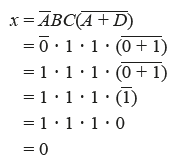
\includegraphics[scale=0.70]{Figuras/algebra_booleana.png}
	\end{center}
    \legend{Fonte: \cite{tocci2003sistemas}}
\end{figure}

\par
Ainda segundo \citeonline{tocci2003sistemas}, devido a esta característica, a álgebra booleana possui três operações básicas, \textit{OR} (ou), \textit{AND} (e) e \textit{NOT} (não). Tal conjunto de operações também é denominado de operações booleanas e, por meio da utilização de tabelas verdade é possível descrever as saídas baseando-se nas entradas e na operação aplicada. Cada operação booleana possui sua tabela verdade (~\autoref{fig:exemplo_diagrama}), bem como sua representação em forma de diagrama.

\begin{figure}[H]
	\begin{center}
    \caption{\label{fig:exemplo_diagrama}Símbolo e tabela verdade para uma porta OR de três entradas.}
	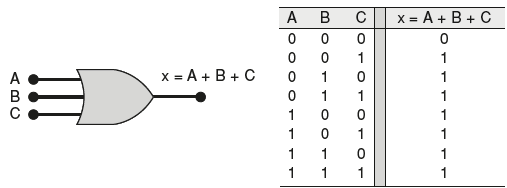
\includegraphics[scale=0.60]{Figuras/exemplo_diagrama.png}
	\end{center}
    \legend{Fonte: \cite{tocci2003sistemas}}
\end{figure}

\begin{figure}[H]
	\begin{center}
    \caption{\label{fig:exemplo_circuito} Representação de circuito lógico, utilizando portas lógicas.}
	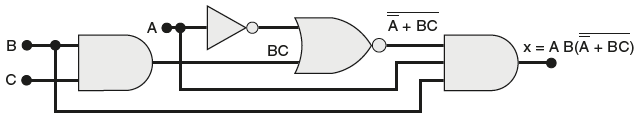
\includegraphics[scale=0.60]{Figuras/exemplo_circuito.png}
	\end{center}
    \legend{Fonte: \cite{tocci2003sistemas}}
\end{figure}

A \autoref{fig:exemplo_circuito} apresenta um circuito lógico formado pelas portas básicas da álgebra booleana. O circuito apresenta três entradas representadas pelas letras A, B e C, mas também formada por duas portas \textit{AND}, uma porta \textit{NOT} e uma porta \textit{OR}. Cada uma destas portas representando operações a serem realizadas, podendo receber como entrada um valor inicial ou resultante de outra porta, como no exemplo ocorre com a última porta \textit{AND}.

\par
\textcolor{red}{Entretanto, segundo \citeonline{kropf2013introduction}, a análise de circuitos é extremamente complexa, resultando em um problema \textbf{NP-Completo}, algoritmos possuem tempo de execução exponencial. Contudo, este tempo de execução exponencial é uma complexidade exponencial para o pior caso, resultando crescimento exponencial da execução a medida que o tamanho do problema aumenta.}

\par
\textcolor{red}{Ainda, segundo \citeonline{kropf2013introduction} a avaliação das funções booleanas podem ser verdadeiras(True) ou falso(False), com isso, para um função com \textit{n} variáveis, apresenta $2^{n}$ possibilidades de avaliação. Utilizando o exemplo da \autoref{fig:exemplo_circuito} que apresenta 3 entradas, logo apresenta 8 possibilidade de avaliação ao final e este número aumenta à medida que o número de variáveis tambeḿ aumenta}

%============================
%VERIFICAÇÃO DE SISTEMAS
%============================
\section{Verificação de sistemas}
 No contexto de verificação de sistemas, faz-se necessário a diferenciação entre verificação e validação. Verificação e validação possuem o intuito de mostrar que determinado sistema funcione conforme o especificado, além de satisfazer as especificações do cliente~\cite{sommerville2011engenharia}. 

\par
Segundo~\citeonline{sargent2005verification}, verificação é o processo de determinar se um modelo computacional obtido por discretização de um modelo matemático de um evento físico e o código que implementa o modelo computacional pode ser usado para representar o modelo matemático do evento com precisão suficiente e validação é o processo de determinar se um modelo matemático de um evento físico representa o evento físico real com precisão suficiente.

\par
A verificação consiste identificação de erros e prováveis problemas que um componente pronto possa apresentar, enquanto a validação busca analisar se tal componente está seguindo os requisitos pré-definidos para sua construção~\cite{koscianski2007qualidade}. O teste de programa, na qual o software  é executado com dados de teste é a principal forma de validação, porém, técnicas de verificação, tais como, inspeção e revisões também podem integrar a etapa de validação~\cite{sommerville2011engenharia}.

\subsection{Diagrama de decisão binária}
Um diagrama de decisão binária(DDB) pode ser definido como um grafo acíclico para representação de funções booleanas. Existe uma ordem rigorosa na ocorrência de variáveis à medida que se percorre o grafo da raiz para a folha. Dado como exemplo a fórmula \textit{f=(a$\lor$b)$\land$(c$\lor$d)} e utilizando a ordenação de variavél $a < b < c < d$, na \autoref{fig:bdd_fig}. Dada a atribuição de valores booleanos as variáveis $a, b, c$ e $d$, pode-se decidir se a atribuição torna a fórmula verdadeira atravessando o início do gráfico na raiz e ramificação em cada nó. Definindo $a,c$ e $d = 1$ e $c = 0$ leva a folha de rótulo 1, portanto, a fórmula é verdadeira para essa tarefa~\cite{clarke1994model}.


\begin{figure}[H]
	\begin{center}
    \caption{\label{fig:bdd_fig}Arvore de decisão binária}
	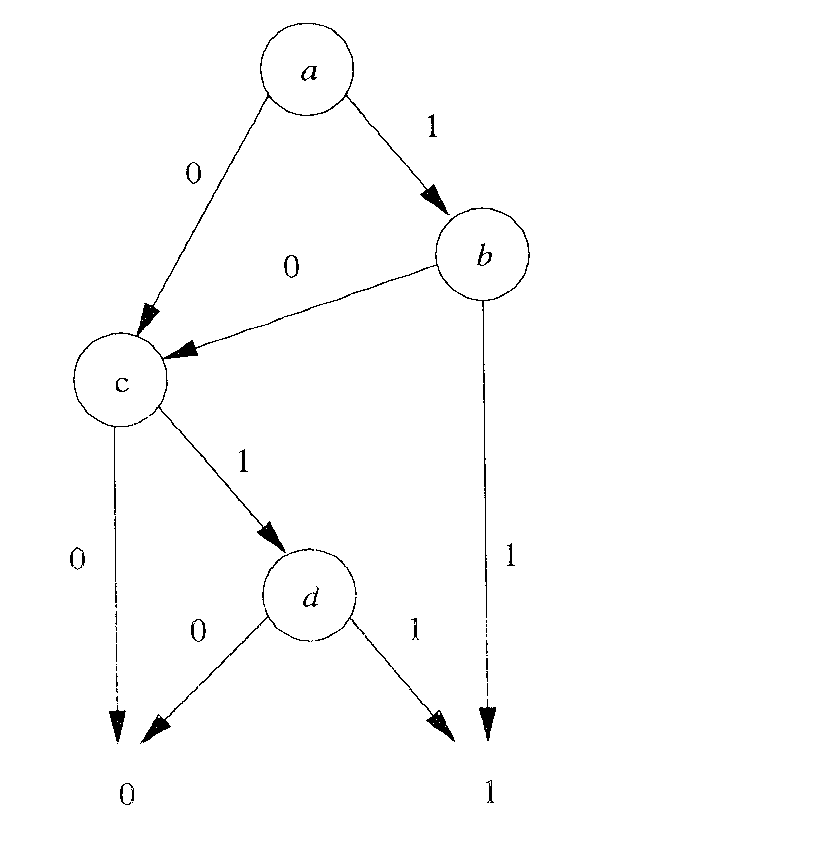
\includegraphics[scale=0.30]{Figuras/Arvore_BDD.png}
	\end{center}
    \legend{Fonte: \cite{clarke1994model}}
\end{figure}

\par
\textcolor{red}{O DDB permite o teste eficiente de satisfabilidade, validade e eficiência \cite{kropf2013introduction}. O uso e DDB em conjunto com \textit{Model Checking} e técnicas de abstração permitiu o aumento na capacidade de verificação, de modo que sistemas mais realistas pudessem ser verificados\cite{biere2003bounded}}

%============================
%MODEL CHECKING
%============================
\subsection{Model Checking}
\par
\textcolor{red}{\textit{Model checking} é uma técnica de verificação formal que explora todos os possíveis estados do sistema, de modo a provar se um modelo satisfaz determinada propriedade. Pode ser aplicada em uma ampla gama de aplicações, tais como sistema embarcados, design de hardware e engenharia de software~\cite{baier2008principles}.}

\par
\textcolor{red}{Entre as vantagens da utilização de \textit{Model Checking} estão:
\begin{itemize}
    \item Possuem suporte a verificação parcial, em outras palavras, a verificação individual de propriedades, permitido foco primeiro as propriedades essenciais\cite{baier2008principles}.
    \item Não requer qualquer interação do usuário, nem um alto grau de especialização para o uso de \textit{model checking}\cite{baier2008principles}.
    \item Possui como base a teoria de grafos, estruturas de dados e lógica no desenvolvimento da solução\cite{baier2008principles}.
    \item Útil para fins de depuração, pois fornece informações em caso de uma propriedade seja invalidada\cite{baier2008principles}.
\end{itemize}}

\par
\textcolor{red}{Por outro lado, apresenta também algumas desvantagens:
\begin{itemize}
    \item Sofre do problema de explosão de espaço de estados, ou seja, a quantidade de estados necessários pode ser maior que a memória disponível pelo sistema\cite{baier2008principles}.
    \item Faz a verificação apenas dos requisitos declarados, logo, não a garantia de integridade. Baseado nisso, a validade de propriedades não verificadas não pode ser julgada\cite{baier2008principles}.
    \item A verificação de modelos geralmente não é computável,  isso deve-se a questões de decidibilidade utilizada \cite{baier2008principles}.
\end{itemize}}

\par
\textcolor{red}{Outras técnicas foram implementadas em conjuntos com \textit{Model checkings} com o intuito de aumentar a capacidade de verificação, como a técnica SAT na qual não sofre do problema de explosão de estados existente usando DDB. A técnica SAT em conjunto com \textit{Model Checking} é conhecida como \textit{Bounded Model Checking} \cite{biere2003bounded}.}

%============================
%BOUNDED MODEL CHECKING
%============================
\subsection{\label{cap:bounded}\textit{Bounded Model Checking}}
Segundo \citeonline{rocha2015verificaccao}, \textit{Bounded Model Checking} (BMC) é um tipo especial de \textit{Model Checking} que usualmente adota o método de satisfabilidade booleana, o qual tem sido introduzido como uma técnica complementar para diagrama de decisão binaria para aliviar o problema da explosão de estados, visto que a técnica de \textit{Model Checking} busca todos os estados possíveis para verificação.

\par
\textit{Bounded Model Checking} é uma técnica para a verificação de uma dada propriedade em uma determinada profundidade do sistema analisado. Logo, dado um sistema de transições M, uma propriedade $\phi$, e um limite (\textit{bound}) $k$, o BMC desenrola o sistema $k$ vezes e traduz o sistema em uma condição de verificação(CV) $\psi$ tal que $\psi$ é satisfeito se e somente se $\phi$ tem um contra-exemplo de profundidade menor ou igual a $k$ \cite{rocha2015verificaccao}.

\par
\textcolor{red}{O \textit{Extended SMT-Based Bounded Model Checker} (ESBMC) é um ferramenta que utiliza técnicas de \textit{Bounded Model Checking} e solucionadores SMT(\textit{Satisfiability Modulo Theories}) para verificação de programas em C/C$++$~\cite{rocha2015model}, permitindo a verificação aritmética de overflow e undeflow, segurança de ponteiros, limite de array e de gerar propriedades de segurança.\cite{cordeiro2012smt,rocha2015verificaccao}.} 
%ESBMC utiliza uma versão modificada do CBMC no \textit{front-end} para analisar o código ANSI-C e para gerar as condições de verificação através de execução simbólica 

\par
No ESBMC, o programa analisado é modelado em um sistema de transição de estados, conforme a trupla: $M=(S,R,S_{0})$, o qual é gerado um grafo de controle de fluxo (GFC), onde $S$ representa o conjunto de estados, $R$ $\subseteq$ $SxS$ representa as transições e $S \subseteq S$ representa o conjuto de estados iniciais. Um estado $s \in S$ consiste no valor do contador de programa (PC) e os valores de todas as variáveis dos programas. O estado inicial $S_{0}$ atribui o inicio do programa GFC ao PC, desta forma o ESBMC identifica as transições, conforme a formula lógica, $\gamma$=($S_{i}$,$S_{i+1}$) que captura as retrições sobre os valores correspondntes do PC e das variáveis do programa~\cite{cordeiro2012smt}.

\par
\textcolor{red}{Segundo o site do ESBMC\cite{esbmc},} a ferramenta permite ao usuário indicar propriedades adicionais\todo{Descrever quais propriedades o esbmc suporta} usando assertivas que também são verificadas. O ESBMC converte as condições usando diferentes técnicas de background\todo{apresentar exemplo} para posteriormente passar para verificador SMT. Outra vantagem é a ferramenta permitir verificação de software single-thread e multi-thread.


\par
\textcolor{red}{O motivo da escolha desta ferramenta, deve-se a mesma ter as funções necessárias para o desenvolvimento do método, como solucionadores SMT, além de premiação em competições, como o SV-COMP, sendo premiado com 2 medalhas de ouro e duas de bronze em 2015 e uma medalha de ouro e uma de prata em 2016~\cite{esbmc}.}

%============================
%REDES DE PETRI
%============================
\subsection{Redes de petri}
\par
\textcolor{red}{Um rede de petri, $N$ é um multigrafo direcionado, ponderado e bipartido, representado pela tupla $N=(P,T,I,O)$, onde $P$ representa um conjunto finito de estados; $T$ representa um conjunto finito de transições.; $I$ representa a função de entrada; e $O$ representa função de saída. Estas funções de entrada e saída determimam o fluxo dos token dentro da rede, sendo dos estados para as transições e das transisções para os estados~\cite{halder2006}.}


\textcolor{red}{Redes de petri são redes baseadas em abstração que pode ser usado como método de modelagem, seja gráfica ou matemática~\cite{halder2006}.}Como ferramenta gráfica são utilizadas como comunicação visual, como fluxogramas, por exemplo, e como ferramenta matemática podem configurar modelos matemáticos que regem o comportamento dos sistemas\cite{murata1989petri}. 

\begin{figure}[htb]
	\begin{center}
    \caption{\label{fig:rede_petri}Rede de petri}
	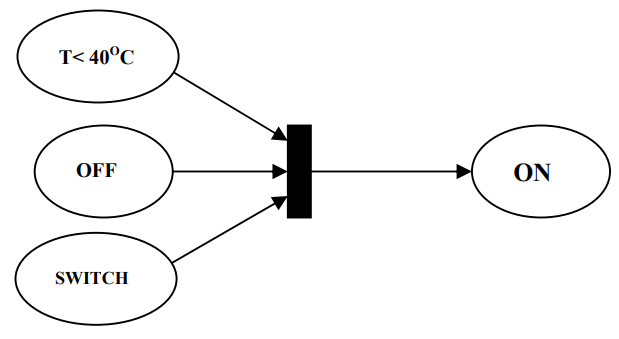
\includegraphics[scale=0.60]{Figuras/rede_petri.png}
	\end{center}
    \legend{Fonte: \cite{halder2006}}
\end{figure}

\par
A \autoref{fig:rede_petri} ilustra a reação quimica: $2H_20 + 0_2 \rightarrow 2H_2O$, onde existe dois token em cada estado inicial, representando que existem duas particulas de $H_2$ e $O_2$ em cada estado. O arco que liga o estado com $H_2$  transição $t$ tem peso 2, isso indica que é necessário dois token deste estado para transição, ocorrendo o mesmo da transição $t$ para o estado $H_2O$, e o estado com $0_2$ é necessário apena um tokem para transição.\cite{murata1989petri}.

\par
Na \autoref{fig:rede_petri}(a) apresenta os tokens todos no estado inicial e a operação pode ser realizada, pois os requisitos para a mesma estão disponivéis, desse caso dois token de $H_2$ e um token de $O_2$. Na \autoref{fig:rede_petri}(b), os tokens são passados a transição $t$ e formando $2H_2O$, seguindo o apresentado na formula. O peso da aresta de saída da transição para o estado seguinte tem peso 2, o que também pode ser realizado e passando dois tokens da transição para o estado $H_2O$\cite{murata1989petri}. 

\par
Após isso, nenhuma operação mais pode ser realizada, devido não conter tokens necessários para a realização da operação representada\cite{murata1989petri}. Esta operação realizada com os tokens é chamado de "\textit{Token game}" que consiste no comportamento da rede de petri, em outras palavras, representa o funcionamento do sistema representado pela rede\cite{halder2006}.

\todo[inline]{\textcolor{blue}{Descrever quais propriedades podem ser verificadas com RP e onde será utilizado no seu trabalho.}}
\par

%============================
%VERIFICAÇÃO DE HARDWARE
%============================
\subsection{Verificação de hardware}

A verificação de hardware, por meio da simulação, visa assegurar que uma implemetação, descrição do hardware em qualquer qualquer nível de abstração da hierarquia de hardware, atinja suas especificações, propriedades que devem ser respeitadas para que a corretude do mesmo seja comprovada~\cite{gupta1992formal}. A Verificação formal de hardware consiste na utilização 
% dos conceitos de verificação formal, mas também 
de técnicas para corretude de circuitos lógicos, ou seja, consiste na utilização de modelos matemáticos para descrição de propriedade e/ou de comportamento de um dado sistema~\cite{kropf2013introduction}.

\par
Entre as abordagens utilizadas na verificação formal de hardware consiste tanto na implementação quanto a especificação estarem descritas em lógica formal, neste caso a corretude será obtida através da comprovada relação entre a implementação e a especificação~\cite{seger1992introduction}. A especificação formal consiste na descrição do comportamento, bem como, das propriedades do sistema em linguagem matemática, tornando-se crucial para o processo de verificação. Na implementação formal, o nível de abstração, tais como, \textit{Gate level} e RTL(\autoref{fig:exemplo_RTL}) são importantes informações para o desenvolvimento do formalismo, bem como as classes, por exemplo se o circuito é sequencial ou combinacional, se utiliza pipeline, etc~\cite{kropf2013introduction}.

\begin{figure}[!htp]
\caption{\label{fig:exemplo_RTL} Exemplo de multiplexador de duas entradas utilizando RTL em VHDL.}
	\begin{center}
    \begin{minipage}{0.7\textwidth}
    \begin{lstlisting}       
library IEEE;
use IEEE.STD_LOGIC_1164.all;

ENTITY mux2 is
  PORT (opt, a, b: in STD_LOGIC;
  f : out STD_LOGIC);
END mux2;

ARCHITECTURE behaviour OF mux2 IS
BEGIN
  PROCESS(opt, a, b)
    BEGIN
        IF opt = '1' THEN
            f <= a;
        ELSE
            f <= b;
        END IF;
    END PROCESS
END behaviour ; 
\end{lstlisting}
    \end{minipage}
	\end{center}
    \legend{Fonte: Própria.}
\end{figure}
\par
A utilização de \textit{Model Checking} também se faz presente nos modelos formais de verificação de hardware, onde apenas é utilizado o comportamento dos circuitos na verificação, de modo a verificar a se as propriedades  presentes são satisfeitas. Para isso, são utilizados os conceitos da lógica proposicional, que por meio da utilização de fórmulas que representem as propriedades dos estados, é possível realizar as verificações necessárias~\cite{seger1992introduction}.

\todo[inline]{Apresentar um exemplo com um circuito e como este pode ser verificando com model checking}
 
%============================
%VERIFICAÇÃO DE SOFTWARE
%============================
\subsection{Verificação formal de software}

% Segundo \citeauthor{rocha2015verificaccao}, o
Observa-se que o uso de verificacão de software tem sido feito aplicado em muitas áreas, tais como, infraestruturas industriais de missão critica e de segurança.  Logo, existe a necessidade de garantir a corretude destes sistemas. Devido a isso, a verificação formal tem sido utilizada em três principais abordagens, sendo elas~\cite{cousot2010gentle,d2008survey}:

\todo[inline]{Apresentar exemplos para os métodos apresentados abaixo}

\begin{itemize}
 \item \textbf{Métodos dedutivos:} Produzem provas matemáticas formais de corretude usando provadores de teoremas ou assistentes de prova para execução da prova e necessitam da interação humana para prover os argumentos~\cite{cousot2010gentle};
  \item \textbf{Verificação de modelos:} Exploram exaustivamente modelos de execuções de programa, que podem ser sujeitos a explosão combinatória, necessário a intervenção humana para geração dos modelos~\cite{rocha2015verificaccao};
  \item \textbf{Analise estática:} Engloba diversas técnicas para calcular automaticamente informações sobre o comportamento de um programa sem executá-lo, sendo utilizado em otimização de código e verificação em compiladres~\cite{d2008survey}.
\end{itemize}

Segundo \citeauthor{rocha2015verificaccao}, na verificação formal de software apresentam-se dificuldades, tais como: quais as propriedades são de interesse na verificação em tempo de execução; e impossibilidade matemática de provar a corretude de propriedades não triviais no comportamento de programas 
% , devido ao computador ser um dispositivo finito
~\cite{cousot2010gentle}. 

%============================
%LÓGICA PROPOSICIONAL
%============================
\subsection{Lógica proposicional}

A lógica proposicional é uma linguagem formal onde é definida um alfabeto e conectivos proposicionais, e um conjunto de regras gramaticais, as quais serão utilizadas para construção das proposições~\cite{souza2017logica}. Porém apesar de importante, ela é limitada, não podendo expressar sentenças elementares importantes, tais como a da aritmética elementar. Por exemplo:
\begin{enumerate}
\item Todos são mortais.
\item Alguém é bondoso.
\end{enumerate}

\textcolor{red}{Na lógica preposicional, não poderiam ser analisadas, pois não teria como decompor ambas em sentença e assim não teria como analisar as diferenças entre ambas. Contudo, no exemplo: "Existem cavalos com patas verdes.", sentença determina que existem cavalos com a caracteristica ou proriedade de terem as patas verde. A relação criada pela frase poderia a ser analisada pela lógica proposicional\cite{abe2002introducao}.}


Segundo \citeauthor{souza2017logica}, alfabeto da lógica proposicional é formado por símbolo de pontuação, símbolos proposicionais e conectivos proposicionais, onde cada um apresenta uma função em específico, sendo:
\begin{itemize}
  \item \textbf{Símbolos de pontuação: }Apenas dois símbolos de pontuação são utilizados o "(" e o ")".
  \item \textbf{Símbolos proposicionais:} São utilizados para representar as proposições, onde um símbolo \textit{P} pode ser utilizado para representar uma proposição qualquer, por exemplo: \textit{P}="Está chovendo". O conjunto de símbolos proposicionais é infinito e enumerável, sendo possível representar infinitos e enumerável conjunto de proposições.
  \item \textbf{Conectivos proposicionais:} São os símbolos usando frequentemente na matemática. Os símbolos recebem a seguinte denominação: 
\begin{enumerate}
\item \textbf{$\neg$}: Representa a partícula de negação, ou seja, "Não".
\item \textbf{$\lor$}: Representa a partícula "Ou"
\item \textbf{$\land$}: Representa a partícula "E"
\item \textbf{$\rightarrow$}: Representa a partícula "Se então ou implica".
\item \textbf{$\Leftrightarrow$}: Representa a partícula "Se, e somente se".
\end{enumerate} 
\end{itemize}

Ainda segundo \citeauthor{souza2017logica}, existem as fórmulas que são constituídas de forma indutiva, a partir de símbolos do alfabeto conforme as regras apresentadas abaixo:
\begin{itemize}
\item Todo o símbolo preposicional é uma fórmula
\item Se \textit{H} é uma fórmula, então ($\neg$\textit{H}), a negação de \textit{H}, é uma fórmula.
\item Se \textit{H} e \textit{G} são fórmulas, então a disjunção de \textit{H} e \textit{G}, dada por (\textit{H} $\lor$ \textit{G}), é uma fórmula.
\item Se \textit{H} e \textit{G} são fórmulas, então a conjunção de \textit{H} e \textit{G}, dada por (\textit{H} $\land$ \textit{G}), é uma fórmula.
\item Se \textit{H} e \textit{G} são fórmulas, então a implicação de \textit{H} e \textit{G}, dada por (\textit{H} $\rightarrow$ \textit{G}), é uma fórmula. Neste caso, \textit{H} é o antecedente e \textit{G} consequente da fórmula.
\item Se \textit{H} e \textit{G} são fórmulas, então a bi-implicação de \textit{H} e \textit{G}, dada por (\textit{H} $\leftrightarrow$ \textit{G}), é uma fórmula. Neste caso, \textit{H} é o lado esquerdo e \textit{G} o lado direito da fórmula.
\end{itemize}


%============================
%Property Specification Language - PSL
%============================
\subsection{Linguagem de especificação de propriedades}
Linguagem de especificação de propriedades, do inglês \textit{Property Specification Language} - PSL, é uma notação formal para especificação de comportamento em sistemas eletrônicos, compatível com as linguagens VHDL\cite{IEEEVHDLLanguage}, Verilog\cite{IEEEVerilogLanguage} e SystemC\cite{IEEESystemCLanguage}. Destina-se a utilização para a especificação funcional, mas também para entrada de ferramentas de verificação. A especificação do PSL é a utilização de assertivas sobre propriedades de um sistema, sendo estas propriedades constituídas de três elementos: expressões boolenas, expressões sequenciais e operadores temporais~\cite{IEEEPSL}.

\par
Segundo \cite{IEEEPSL}, o PSL foi totalmente desenvolvida com o intuito fornecer leitura e escrita de fácil entendimento, sintaxe concisa, semântica formal e rigorosamente bem definida e ser matematicamente precisa, visto a utilização da mesma em processo de verificação. 

O PSL pode ser utilizado para capturar requisitos relativos ao comportamento total do projeto, bem como, sobre o modo que o mesmo deverá operar no ambiente, ms também para capturar requisitos comportamentais e os pressupostos que surgem durante o processo de design. Ambas podem ser utilizadas para verificação de sistemas. 

\textcolor{red}{O PSL possui 4 camadas, sendo:
\begin{itemize}
    \item \textbf{Camada booleana:} É utilizada para criar as expressões que são usadas pelas outras camadas. As expressões de camada booleana são avaliadas em um único ciclo de avaliação e obedecem as caracteristicas da linguagem na qual foi escrita. Na \autoref{fig:psl_example1} apresenta um expressão \textit{if} usando PSL nas linguagens VHDL e Verilog\cite{IEEEPSL}.
    \item \textbf{Camada temporal:} É usado para descrever as propriedades do circuito. Pode descrever propriedades envolvendo relações temporais e são avaliadas em uma serie de ciclos de avaliação. Na \autoref{fig:psl_example2} apresenta a estrutura \texttt{@clk}, permitindo que determinda operação seja executada em tempos especificos de execução ou em cilcos especificos.\cite{IEEEPSL}.
    \item \textbf{Camada verificação:} É usada para informar de que modo as propriedades na camada temporal devem ser utilizadas pelas ferramentas de verificação. Na \autoref{fig:psl_example3} apresenta o uso de \textbf{assert} que busca provar a proriedade e \textbf{assume} que a ferramenta deve assumir como verdadeiro a propriedade~\cite{IEEEPSL}.
    \item \textbf{Camada de modelagem:} É usada para modelar comportamento de entradas, no caso de ferramentas que não utiizem casos de teste e para modelar circuitos adicionais para verificação, mas que não fazem parte do circuito principal\cite{IEEEPSL}.
\end{itemize}
}
\begin{figure}[H]
\caption{\label{fig:psl_example1} Exemplo de PSL em VHDL e Verilog.}
	\begin{center}
    \begin{minipage}{0.7\textwidth}
    \begin{lstlisting}       
    (a &   (a-1)) == 0         // Verilog
    (a and (a-1)) =  0         -- VHDL
    \end{lstlisting}
    \end{minipage}
	\end{center}
    \legend{Fonte: \cite{duolos2018}}
\end{figure}

\begin{figure}[H]
\caption{\label{fig:psl_example2} Exemplo da camada temporal em PSL.}
	\begin{center}
    \begin{minipage}{0.7\textwidth}
    \begin{lstlisting}       
    (always req -> next (ack until grant)) @clk
    \end{lstlisting}
    \end{minipage}
	\end{center}
    \legend{Fonte: \cite{duolos2018}}
\end{figure}

\begin{figure}[H]
\caption{\label{fig:psl_example3} Exemplo da camada de verificação em PSL.}
	\begin{center}
    \begin{minipage}{0.7\textwidth}
    \begin{lstlisting}       
    vunit my_properties(myVerilog.instance.name){
    assert (always req -> ack) @ clk;
    assume (never req && reset)@ clk;
    }
    \end{lstlisting}
    \end{minipage}
	\end{center}
    \legend{Fonte: \cite{duolos2018}}
\end{figure}

%============================
%Assertion-based verification - ABV
%============================

\subsection{Verificação baseada em assertivas}

Verificação baseada em assertivas, do inglês \textit{Assertion-Based Verification} - ABV, é um paradigma de verificação igualmente adequado para verificação formal e abordagens baseadas em simulação~\cite{boule2005incorporating} e em conjunto com a tecnica de PSL tem ganhado aceitação como um método essencial para verificação funcional do hardware~\cite{DahanCombining}.

\par
\textcolor{red}{Na ABV as assertivas são declaração adicionadas ao projeto com o intuito de especificar o comportamento do projeto~\cite{boule2005incorporating}, podendo escritos em PSL ou em SVA (\textit{System Verilog Assertions}). No caso deste projeto será utilizado a PSL, devido a mesma ser utilizada juntamente com a linguagem VHDL. Com a utilização de ABV o circuito pode ser verificado usando técnicas de simulação e/ou verificação, por exemplo, \textit{model checking}, para garantir que o mesmo esteja de acordo com o pretendido projeto~\cite{DahanCombining}.}

\par
\textcolor{red}{Na \autoref{fig:assertiva} apresenta o modelo de assertiva utilizada no projeto, utilizando de um modelo próprio para assertivas, unindo as funcionalidades já existentes nas assertivas do VHDL, mas também novas (serão apresentadas nas próximas seções), fornecendo assim mais propriedades a serem analisadas. A assertiva apresentada na \textbf{linha 13} da \autoref{fig:assertiva_abv} faz a verificação se a porta AND, ao ter entradas de dois valores 1, a saída também será 1, caso não seja será relatado erro de verificação.}

\begin{figure}[H]
\caption{\label{fig:assertiva_abv} Exemplo de declaração de assertiva no VHDL.}
	\begin{center}
    \begin{minipage}{0.9\textwidth}
    \begin{lstlisting}       
library ieee;
use ieee.std_logic_1164.all;
entity AND_ent is
port(   x,y: in bit;
        F: out bit
);
end AND_ent;

architecture behav1 of AND_ent is
begin
	--@c2vhdl:ASSERT
    --assert (F='0')
    --report "O valor de F é diferente de 1"
    --severity ERROR;
    --@c2vhdl:END
	process(x, y)
    	begin
        	if ((x='1') and (y='1')) then
            	F <= '1';
        	else
            	F <= '0';
        	end if;
    	end process;
end behav1;

\end{lstlisting}
    \end{minipage}
	\end{center}
    \legend{Fonte: Própria.}
\end{figure}

%============================
%PROPRIEDADES DE SEGURANÇA
%============================
\subsection{Propriedades de segurança}

Propriedades de segurança é um meio de validação do comportamento de um determinado sistema, de modo que se uma dada propriedade de segurança for violada, então através de uma execução finita, é possível verificar tal erro. Algumas propriedades de segurança, no entanto, podem impor requisitos em fragmentos de caminho finito e não podem ser verificadas considerando apenas os estados alcançáveis. \cite{baier2008principles}.

\par
Segundo \cite{clarke2003verification}, podemos definir uma propriedade de segurança como: \textit{dado um sistema de transições $ST = (S, S_0, E)$, seja um conjunto $B \subset S$ que especifica um conjunto de maus estados tais que $S_0 \cap B = \emptyset$, pode-se dizer que $ST$ é seguro com relação a $B$, denotado por $ST \models AG\neg B$ se não existe um caminho no sistema de transição do estado inicial $S_0$ até o estado $B$, de outro modo é dito que $ST$ não é seguro}.

\todo[inline]{\textcolor{yellow}{Adicionar exemplos de propriedades de segurança em hardware.}}


%============================
%TECNICAS DE COMPILADORES
%============================
\section{Técnicas de compiladores}
\par
Compiladores são sistemas de software utilizados para tradução de uma linguagem de programação para outra, ou seja, o programa da linguagem fonte é lido e traduzido para um código equivalente na outra linguagem, ou linguagem alvo. Geralmente utilizada para transformar trechos de código em uma linguagem a ser executada pelo computador~\cite{aho2007compilers}. 

\par
Diversas técnicas podem ser utilizadas nas diversas etapas, até que o código seja traduzido, tais como LL(1) e LR na análise sintática; eliminação de código morto; propagação de constante e \textit{Peephole} na otimização de código~\cite{aho2007compilers}. Neste projeto serão focados as áreas de transformações de código e otimização de código.
99346385
%============================
%TRANSFORMAÇÕES DE CÓDIGO
%============================
\subsection{Transformações de código}
\par
Transformações de código correspondem a uma complexa função que envolve analise de fluxo de dados e modificação completa do programa que são parte integral da alta performance e sistemas computacionais. Podem ser classificados em transformações escalares que reduzem o número de instruções a serem executadas no programa ou transformações paralelas que maximizam o paralelismo~\cite{srikant2002compiler}.

\par
A \autoref{fig:cod_vhdl} representa o trecho de código apresentado na \autoref{fig:assertiva}. O trecho representa o comportamento das entradas, neste caso de um código da porta \texttt{AND}. E a figura \autoref{fig:cod_c} representa a tradução deste trecho em código na linguagem C. Esta tradução foi realizada pela ferramenta V2C~\cite{albertoV2C}, utilizada neste projeto.

\begin{figure}[thp]
\caption{\label{fig:cod_vhdl} Trecho de código em VHDL representando porta \texttt{AND}.}
	\begin{center}
    \begin{minipage}{0.9\textwidth}
    \begin{lstlisting}       
	process(x, y)
    	begin
        	if ((x='1') and (y='1')) then
            	F <= '1';
        	else
            	F <= '0';
        	end if;
    	end process;
\end{lstlisting}
    \end{minipage}
	\end{center}
    \legend{Fonte: Própria.}
\end{figure}

\begin{figure}[thp]
\caption{\label{fig:cod_c} Trecho de código traduzido para linguagem C.}
	\begin{center}
    \begin{minipage}{0.9\textwidth}
    \begin{lstlisting}       
   /* Start of Translation */
   /* p0: */
   if (chg[x] || chg[y]) {
      if (((old[x]==1) && (old[y]==1))) {
      	new[f]=1;
      }
      else {
      	new[f]=0;
      }
   }
   /* End of Translation */

	\end{lstlisting}
    \end{minipage}
	\end{center}
    \legend{Fonte: Própria.}
\end{figure}

\todo[inline]{Expandir esta seção. Apresentar propriedades de transformação e técnicas para avaliar a transformação}

%============================
%OTIMIZAÇÃO ok
%============================
\subsection{Otimização de código}
\par
A otimização de código consiste na melhoria do código intermediário gerado pelos algoritmos de compilação com o objetivo de obter um menor tempo de execução do programa, porém outros fatores podem ser introduzidos, como algoritmos menores. Este fato não implica em afirmar que o melhor código é gerado, visto que dada a complexidade, raramente pode ser obtido que o código gerado pode ser o melhor possível~\cite{aho2007compilers}.

\par
Segundo \citeauthor{aho2007compilers}, otimização local de código consiste na otimização de um bloco básico de código, ou seja, a otimização ocorre em um trecho especifico de código. Os blocos básicos são trecho onde não ocorrem saltos ou \textit{loops}, para nenhuma outra parte do código. A otimização global de código é baseado na analise do fluxo de dados, de modo que ocorra as elminação de instruções não necessárias ou substituição mais facil. A otimização global consite na analise completa do código. Neste sentido, nas próximas seções serão apresentadas algumas importantes técnicas de otimizações.

%============================
%Grafo Acliclico Direcional - GAD ok
%============================
\subsubsection{Grafo Acliclico Direcional - GAD}
\par
Grafo Aciclico Direcional é utilizado para diversos fins dentro da estrutura de compiladores, principalmente para geração da \textit{parse tree} otimização de código. Pode ser usado na representação de instruções unicas blocos básicos de código\cite{aho2007compilers}. O uso de GAD permite a melhoria de de código, tais como:
\begin{itemize}
\item Elminação de subexpressões locais comuns, ou seja, expressões que o valor já foi computado anteriomente;
\item Eliminação de código morto;
\item  Reordernamento de declarações buscando reduzir o tempo que o valor temporário necessita ser preservado em um registro;
\end{itemize}

\par
\begin{figure}[thp]
\caption{\label{fig:basic_block} Exemplo de bloco basico de código.}
	\begin{center}
    \begin{minipage}{0.9\textwidth}
    \begin{lstlisting}
    a = b + c
    b = a - d
    c = b + c
    d = a - d
	\end{lstlisting}
    \end{minipage}
	\end{center}
    \legend{Fonte: \cite{aho2007compilers}}
\end{figure}

\begin{figure}[htb]
	\begin{center}
    \caption{\label{fig:gda}GAD do bloco básico da \autoref{fig:basic_block}}
	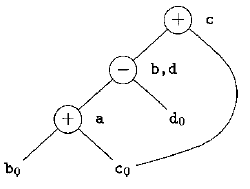
\includegraphics[scale=0.70]{Figuras/GDA.png}
	\end{center}
    \legend{Fonte: \cite{aho2007compilers}}
\end{figure}

A \autoref{fig:basic_block} apresenta um bloco básico com algumas instruções, no caso apresentando são $4$ operações entre somas e multiplicação e a partir deste bloco a \autoref{fig:gda} apresenta o GDA deste trecho de código. Nele apresenta cada nó como uma operação especifica e os terminais como as parcelas das operações.


%============================
%Grafo de Fluxo de Controle - GFC 
%============================
\subsubsection{Grafo de Fluxo de Controle - GFC}

Grafo de fluxo de controle corresponde a um grafo direcionado, no qual cada nó representa blocos básicos e cada aresta representa os caminhos de fluxo entre os blocos basicos~\cite{allen1970control}. É importante ressaltar que saltos determinam o final de um determinado bloco básico, ou seja, saltos indicam um caminho para uma nova região de código básico~\cite{aho2007compilers}.

\par
\textcolor{red}{Conforme apresentado, na \autoref{fig:cfg_example}(a) apresenta um código dividido em blocos, onde cada bloco apresenta estrutura de decisão \textit{if}. Cada bloco, seja para caso verdadeiro(\textit{True}, ou seja para caso (\textit{False}), é definido por um bloco, dessa forma o grafo de fluxo pode ser gerado. Na \autoref{fig:cfg_example}(b), apresenta um dos possivéis caminho de execução de código, baseando-se nos resultados gerado pelas estruturas de condição.}

\begin{figure}[H]
	\begin{center}
    \caption{\label{fig:cfg_example}Exemplo da utilização de GFC}
	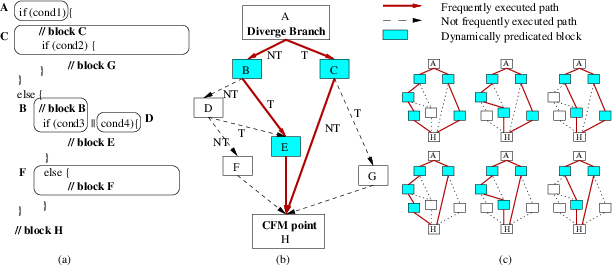
\includegraphics[scale=1.2]{Figuras/cfg_example.png}
	\end{center}
    \legend{Fonte: Adaptado \cite{kim2006diverge}}
\end{figure}

%============================
%Analise do fluxo de dados ok
%============================
\subsubsection{Análise do fluxo de dados}
\par
Análise de fluxo de dados refere-se ao conjunto de técnicas que derivam informações sobre o fluxo de dados ao longo dos caminhos de execução do programa. Para análise do programa, é necessário considerar todas as posiveis execuções através do grafo de fluxo de controle~\cite{aho2007compilers}.

\par
\textcolor{red}{Na \autoref{fig:cfg_example}(c), mostra todas as possivéis execuções do código gerdas a partir do grafo de fluxo de controle. Dsta forma, através dessa análise, é possivél determinar se um código ou trecho de código pode ser eliminado, assim melhorando a execução do código\cite{aho2007compilers}.}
%============================
%Eliminção de código morto 
%============================
\subsubsection{Eliminção de código morto}

A eliminacação de código morto é uma técnica que busca a eficiência de um programa evitando a execução de instruções não necessária em tempo de execução~\cite{knoop1994partial}. O código morto consiste em instruções que não serão alcançáveis durante o fluxo do programa, sendo esta técnica basicamente a  retirada de qualquer variável que não será utilizada em qualquer outro nó do grafo~\cite{aho2007compilers}.

\par
A utilização de GAD corresponde na eliminação de qualquer nó raiz, ou seja, nó sem ancestrais, as quais não esteja ativa anexada a mesma. A execução repetida desta operação removerá todos os nós correspondentes a código morto~\cite{aho2007compilers}.

\begin{figure}[H]
	\begin{center}
    \caption{\label{fig:elimicacao_codigo}GAD do bloco básico da \autoref{fig:basic_block}}
	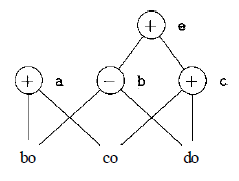
\includegraphics[scale=0.70]{Figuras/eliminacao_codigo.png}
	\end{center}
    \legend{Fonte: \cite{aho2007compilers}}
\end{figure}

Na \autoref{fig:elimicacao_codigo}, supondo que os nós $a,b$ e $c$ estejam ativa, porém o nó é não esteja, o último pode ser eliminado imediatamente. Os nós restantes continuam no GDA, a menos que não tenho variáveis ativas atreladas aos nós~\cite{aho2007compilers}.

%============================
%Gerador de código ok
%============================
\subsubsection{Gerador de código}
\par
O gerador de código é responsavél pela tradução final do programa-fonte para o programa-alvo, o mesmo recebe como entrada um código intermediário juntamente com a tabela de símbolos. Faz-se necessário que o programa-fonte tenha sido analisado sintatica e lexicamente, assim evitando que erros possam ser passados para o programa-alvo, por outro lado a existência de uma nível de otimização, faz-se opicional neste caso~\cite{aho2007compilers}.

\par
O gerador de código possui três tarefas primarias, sendo as mesmas seleção de instrução, alocação de registros e atribuições. A seleção de instruções envolve a escolha das instruções apropriadas da máquina-alvo para implementar as declarações do código intermediario. A atribuição e atribuição de registros envolve a decisão sobre os valores a serem registrados nos registros\cite{aho2007compilers}.

\todo[inline]{Apresentar exemplo}
